%% Einleitung

\begin{tabularx}{\textwidth}{Xr}
  Constantin Lazari, Marco Wettstein & \today\\
\end{tabularx}

%% Fragen
\begin{questions}
	\titledquestion{Kodieren Sie die gegebenen Zeichen mit UTF-8.}
	\thequestiontitle
	\begin{parts}
		\part \enquote{y}
		\begin{solutionordottedlines}[2cm]
			Für UTF-8 gelten die folgende Kennzahlen, sowie: Folgebyte Präfix: 10\\
			\begin{tabular}{lccccccc}
						& 1 Wort 	& ~~~	& 2 Wörter 	& ~~~ 	& 3 Wörter 	& ~~~ 	& 4 Wörter \\
			Präfix 		& 0		&		& 110		&		& 1110		&		& 1111\,0  \\
			Freie Bits	& 7		&		& 11		&		& 16		&		& 21 \\
			\end{tabular}\\
			$y \in \mbox{ASCII}: \mathrm{y}_{\mbox{\scriptsize ASCII}} = 79_{16} = 111\,1001_2 $ (7 Bits) $\rightarrow \mathrm{y}_{\mbox{\scriptsize UTF-8}} = 0111\,1001_2$  
		\end{solutionordottedlines}
		
		\part \enquote{\euro}
		\begin{solutionordottedlines}[2cm]
			Für die Bits-Wörter Tabelle siehe Lösung (a).\\
			\enquote{\euro} gehört nicht zum ASCII Zeichensatz. Gemäss Unicode-Tabelle:\\
			$\mbox{\euro}_{\mbox{\scriptsize Unicode}} = 20\mathrm{AC}_{16} = 10\,0000\,1010\,1100_{16}$ (14 Bits)\\
			Für 14 Bits werden gemäss Tabelle drei Wörter benötigt, das erste mit Präfix \enquote{1110}, die weiteren jeweils mit Präfix \enquote{10}. 
			Das Euro-Zeichen benötigt nur 14 statt 16 Bits, deshalb wird nach dem ersten Präfix noch \enquote{00} eingefügt: \\
			$\rightarrow \mbox{\euro}_{\mbox{\scriptsize UTF-8}} = 1110\,0010:1000\,0010:1010\,1100_2$
		\end{solutionordottedlines}
		
	\end{parts}

	%%%%%%%%%%%%%%%%%%%%%%%%%%%%%%%%%%%%%%%%%%%%%%%%%%%%

	\titledquestion{Geben sei der folgende Code $K = \{0010, 1000, 100, 110\}$. Dieser Code ist weder zyklisch noch präfixfrei.}
	\thequestiontitle
	\begin{parts}
		\part Warum ist $K$ weder zyklisch noch präfixfrei?
		\begin{solutionordottedlines}[2cm]
			Er ist nicht zyklisch, weil in $110$ zweimal die $1$ vorkommt, in $100$ hingegen nur einmal.

			Er ist nicht präfixfrei, weil $100$ den gleichen Anfang hat wie $1000$. $100$ ist in $1000$ enthalten.
		\end{solutionordottedlines}
		
		\part Welche Codewörter in $K$ müssen mindestens entfernt werden, damit K präfixfrei ist?
		\begin{solutionordottedlines}[2cm]
			Entweder $100$ oder $1000$.
		\end{solutionordottedlines}
		%\pagebreak
		\part Welche Codewörder in $K$ müssen mindestens hinzugefügt werden, damit K ein zyklischer Code ist?
		\begin{solutionordottedlines}[2cm]
			$0100, 0001, 010, 001, 101, 011$
		\end{solutionordottedlines}
	\end{parts}

	%%%%%%%%%%%%%%%%%%%%%%%%%%%%%%%%%%%%%%%%%%%%%%%%%%%%
	\titledquestion{Bestimmen Sie den Hamming-Abstand für folgende Paare von Wörtern.}
	\thequestiontitle

	\begin{parts}
		\part \enquote{1110\,0110} und \enquote{1010\,0111} (binär betrachten)
		\begin{solutionordottedlines}[2cm]
			Anmerkung: Für den Hamming-Abstand spielt die Anzahl der Buchstaben im Alphabet keine Rolle.\\
			$1\underline{1}10\,011\underline{0} \mbox{~und~} 1\underline{0}10\,011\underline{1} \rightarrow \mbox{Hamming Abstand}=2$\\
		\end{solutionordottedlines}
		
		\part \enquote{1334} und \enquote{1332} (als Ziffern betrachten)
		\begin{solutionordottedlines}[2cm]
			Anmerkung: Für den Hamming-Abstand spielt die Anzahl der Buchstaben im Alphabet keine Rolle.\\
			$133\underline{4} \mbox{~und~} 133\underline{2} \rightarrow \mbox{Hamming-Abstand}=1$
		\end{solutionordottedlines}

		\part \enquote{Abba} und \enquote{Baba} (als Zeichen betrachten)
		\begin{solutionordottedlines}[2cm]
			Anmerkung: Für den Hamming-Abstand spielt die Anzahl der Buchstaben im Alphabet keine Rolle.\\
			\underline{Ab}ba und \underline{Ba}ba $\rightarrow$ Hamming-Abstand$=2$
		\end{solutionordottedlines}
	\end{parts}

	%%%%%%%%%%%%%%%%%%%%%%%%%%%%%%%%%%%%%%%%%%%%%%%%%%%%
	\pagebreak
	\titledquestion{Gegeben sei ein Alphabet $Z = {A, B, C, D, E, F, G}$ mit:\\
		$p(A) = 0{,}36, p(B) = 0{,}22, p(C)= 0{,}18, p(D) = 0{,}18, $\\
		$p(E) = 0{,}03, p(F) = 0{,}02, p(G) = 0{,}01$} 
	\thequestiontitle

	\begin{parts}
		\part Bestimmen Sie die Entropie ($\sum_{i=1}^n p_i \cdot I_i$) eines Zeichens von Z
		\begin{solutionordottedlines}[2cm]
			\begin{equation*}
				H_Z = \sum_{i=1}^n p_i \cdot I_i = - \sum_{i=1}^n p_i \cdot \log_2 p_i
			\end{equation*}
			\begin{multline*}
				= (0{,}36 \cdot \log_2 0{,}36) 
					+ (0{,}22 \cdot \log_2 0{,}22) 
					+ (0{,}18 \cdot \log_2 0{,}18)
					+ (0{,}18 \cdot \log_2 0{,}18)\\ 
					+ (0{,}03 \cdot \log_2 0{,}03)
					+ (0{,}02 \cdot \log_2 0{,}02) 
					+ (0{,}01 \cdot \log_2 0{,}01)
					\approx 2{,}2329
			\end{multline*}
			Die Entropie ist für alle Zeichen gleich, nämlich ungefähr $2{,}2329$
		\end{solutionordottedlines}

		\part Geben Sie eine mögliche Kodierung für die Zeichen von $Z$ unter Verwendung
		\begin{subparts}
			\subpart einer Gleichverteilung
			\begin{solutionordottedlines}[2cm]
				Das Alphabet besteht aus 7 Zeichen, also werden aufgrund von $\lceil n \rceil = \log_2 |Z|$ mit $|Z| = 7$ mindestens 3 Bits benötigt.
				Eine mögliche Kodierung ist dann:\\
				\begin{tabular}{lclclcl}
					A = 001 & ~~~ & B = 010 & ~~~ & C = 011 & ~~~ & D = 100 \\
					E = 101 & ~~~ & F = 110 & ~~~ & G = 111 & & \\
				\end{tabular}
			\end{solutionordottedlines}

			\subpart dem Shannon-Fano Algorithmus
			\begin{solutionordottedlines}[2cm]
			\begin{enumerate}
				\item $G_{1A} = \{A, D\}: p = 0{,}54$,\\ $ G_{1B} = \{B, C, E, F, G\}: p = 0{,}46$ (Erstes Bit)
				\item $G_{2AA} = \{A\}: p = 0{,}36$,\\$ G_{2AB} = \{D\}: p = 0{,}18$\\
					$G_{2BA} = \{B, G\}: p = 0{,}23$,\\$ G_{2BB} = \{C, E, F\}: p = 0{,}23$ (Zweites Bit)
				\item $G_{3BAA} = \{B\}: p = 0{,}22, G_{2BAB} = \{G\}: p = 0{,}01$\\
					$G_{3BBA} = \{C\}: p = 0{,}18, G_{3BBB} = \{E, F\}: p = 0{,}05$ (Drittes Bit)
				\item $G_{4BBBA} = \{E\}: p = 0{,}03, G_{4BBBB} = \{F\}: p = 0{,}02$ (Viertes Bit)
			\end{enumerate}
			Daraus folgt, als eine mögliche Kodierung:\\
				\begin{tabular}{lclclcl}
					A = 00 & ~~~ & B = 100 & ~~~ & C = 110 & ~~~ & D = 01 \\
					E = 1110 & ~~~ & F = 1111 & ~~~ & G = 101 & & \\
				\end{tabular}
			\end{solutionordottedlines}
			
			\pagebreak
			\subpart dem Huffman Algorithmus an
			\begin{solutionordottedlines}[2cm]
				\begin{enumerate}
					\item $G_1 = \{F, G\}: p = 0{,}03$
					\item $G_2 = \{E\{F, G\}\}: p = 0{,}06$
					\item $G_3 = \{D,\{E\{F, G\}\}\}: p = 0{,}24$
					\item $G_4 = \{B, C\}: p = 0{,}40$
					\item $G_5 = \{A,\{D,\{E\{F, G\}\}\}\}: p = 0{,}60$
					\item $G_6 = \{\{B, C\}, \{A,\{D,\{E\{F, G\}\}\}\}\}: p = 1{,}00$
				\end{enumerate}
			Oder als Baum:\\
			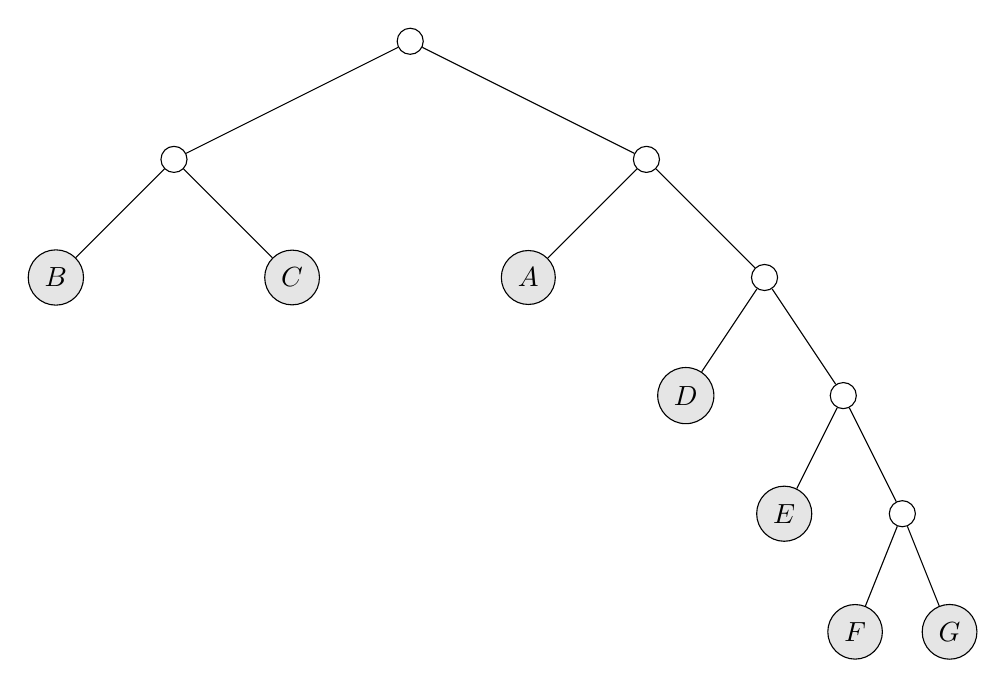
\begin{tikzpicture}[
				level/.style={sibling distance=60mm/#1},
				leaf/.style={circle, draw=black, fill=black!10},
				node/.style={circle, draw=black}
				]
			\node [node] {}
				child {node [node] {}
					child{node [leaf] {$B$}}
					child{node [leaf] {$C$}}
				}
				child {node [node] {}
					child{node [leaf] {$A$}}
					child{node [node] {}
						child{node [leaf] {$D$}}
						child{node [node] {}
							child{node [leaf] {$E$}}
							child{node [node] {}
								child{node [leaf] {$F$}}
								child{node [leaf] {$G$}}
							}
						}
					}
				};
			\end{tikzpicture}\\
			Daraus folgt, als eine mögliche Kodierung:\\
				\begin{tabular}{lclclcl}
					A = 10 & ~~~ & B = 00 & ~~~ & C = 01 & ~~~ & D = 111 \\
					E = 1101 & ~~~ & F = 11110 & ~~~ & G = 11111 & & \\
				\end{tabular}
			\end{solutionordottedlines}

		\end{subparts}

	\end{parts}

	%%%%%%%%%%%%%%%%%%%%%%%%%%%%%%%%%%%%%%%%%%%%%%%%%%%%
	\pagebreak
	\titledquestion{Gegeben sei das Alphabet $Z = \{A, B, C\}$, mit $p(A)= 0{,}4$, $p(B)= 0{,}1$ und $p(C)= 0{.}5$}
	\thequestiontitle

	\begin{parts}
		\part Geben Sie eine mögliche Codierung für das Wort \enquote{AAC} mit der arithmetischen Kodierung an
		\begin{solutionordottedlines}[2cm]
			\begin{enumerate}
				\item Startintervall sei $I_0 = [0,1)$
				\item Aufgrund der Häufigkeiten gelten folgende Teilintervalle:\\
				\begin{tabular}{lclcl}
					$I_a = [0, 0{,}4)$ & ~~~ & $I_b = [0{,}4, 0{,}5)$ & ~~~ & $I_c = [0{,}5, 1)$ 
				\end{tabular}
				\item Erstes Zeichen: \enquote{A} liegt im Interval $I_a = [0, 0{,}4)$
				\item $I_a$ nach Häufigkeiten unterteilt ergibt:\\
				\begin{tabular}{lclcl}
					$I_a = [0, 0{,}16)$ & ~~~ & $I_b = [0{,}16, 0{,}2)$ & ~~~ & $I_c = [0{,}2, 0{,}4)$ 
				\end{tabular}
				\item Zweites Zeichen: \enquote{A} liegt im Interval $I_a = [0, 0{,}16)$
				\item $I_a$ nach Häufigkeiten unterteilt ergibt:\\
				\begin{tabular}{lclcl}
					$I_a = [0, 0{,}064)$ & ~~~ & $I_b = [0{,}064, 0{,}08)$ & ~~~ & $I_c = [0{,}08, 0{,}16)$ 
				\end{tabular}
				\item Drittes Zeichen: \enquote{C} liegt im Intervall $I_c = [0{,}08, 0{,}16]$
				\item Kürzesten Wert aus $I_c = [0{,}08, 0{,}16]$ wählen: $0{,}1$
			\end{enumerate}
			Eine mögliche Kodierung für \enquote{AAC} ist $0{,}1$.
		\end{solutionordottedlines}
		
		\part Wieso gibt es mehrere / viele Möglichkeiten für eine Codierung von \enquote{AAC} mit der arithmetischen Kodierung?
		\begin{solutionordottedlines}[2cm]
			Bei der arithmetischen Kodierung werden Intervalle bestimmt um ein Wort zu kodieren. 
			Das kodierte Wort liegt dann in einem berechneten Intervall.
			Da ein Intervall immer unendlich viele Werte enthält, gibt es unendlich viele mögliche Kodierungen.
		\end{solutionordottedlines}

	\end{parts}

	%%%%%%%%%%%%%%%%%%%%%%%%%%%%%%%%%%%%%%%%%%%%%%%%%%%%

\end{questions}

